\documentclass[11pt]{article}

\usepackage[margin=1in]{geometry}
\usepackage{setspace}
\usepackage{graphicx}
\usepackage{booktabs}
\usepackage{amsmath, amssymb}
\usepackage[numbers]{natbib}
\usepackage{hyperref}
\usepackage{float}
\usepackage{indentfirst}
\setlength{\parindent}{2em}
\onehalfspacing

\title{Performance Evaluation for Multimodal Model}
\author{Guanyi Wu}
\date{}

\begin{document}

\maketitle

\begin{abstract}
This study evaluates multimodal survival models' prediction performance for cancer outcomes. The analysis focuses on three major components: prediction accuracy, variable contribution and prediction uncertainty. In the first section, we compare Cox proportional hazards model and random survival forest (RSF) models using the inverse probability of censoring weighting Brier score. Then we  measure the contribution of each variable based on integrated Brier score. Finally, we construct prediction intervals for estimated median survival time using conformal inference. In general, these methods provide a comprehensive framework for evaluating survival prediction models under right censoring.
\end{abstract}

\section{Introduction}

Accurate prediction of survival outcomes is an important part in cancer research. Reliable survival prediction can help identify high-risk patients, support treatment planning, and improve individual clinical decision. However, survival outcomes are difficult to model because many data are right-censored. In this situation, the exact survival time is not observed and tranditional estimators are ususally biased. Therefore, both model fitting and model evaluation should account for censoring.

The Cox proportional hazards model is a classical method for survival analysis. It provides interpretable regression coefficients and hazard ratios, but it may not capture nonlinear effects. Random survival forests provide a more flexible framework. RSF models extend random forests to right-censored survival data and can estimate patient-specific survival curves without specifying a parametric hazard function \citep{ishwaran2008random}.

This study uses clinical variables, including age, gender, cancer stage, and cancer type, together with mutation indicators for TP53, KRAS and EGFR. Our objective is to evaluate the prediction performance of survival models. As mentioned before, survival prediction is affected by censoring, so prediction performance should be evaluated by methods designed for survival data. The IPCW Brier score provides a reliable way to evaluate prediction error under censoring \citep{gerds2006consistent}. In addition, to quantify the uncertainty of estimation, we use conformal inference  to construct prediction intervals \citep{lei2018distribution}.

% The main objectives of this report are:
% \begin{enumerate}
%     \item To compare the time-dependent prediction accuracy of Cox and RSF models.
%     \item To evaluate which predictors contribute most to survival prediction.
%     \item To quantify uncertainty in predicted median survival time using conformal prediction intervals.
% \end{enumerate}

\section{Methods}

\subsection{Data Processing}

The analysis uses patient-level data containing survival outcomes, clinical variables, and mutation information. The outcome variable is overall survival time, measured in months. Let $T_i$ denote the observed follow-up time for patient $i$, and $\delta_i$ denote the event indicator:
\[
\delta_i =
\begin{cases}
1, & \text{if death was observed},\\
0, & \text{if the observation was right-censored}.
\end{cases}
\]

Mutation indicators were constructed at the patient level, where 1 means that the patient had a somatic mutation in the corresponding gene and 0 means that no such mutation was observed. For unknown mutation information, we assume it to be 0.

\subsection{Modeling}

Two survival models were considered in our analysis. The first model was the Cox proportional hazards model:
\[
h(t \mid X_i) = h_0(t)\exp(\beta^T X_i),
\]
where $h_0(t)$ is the baseline hazard and $X_i$ is the covariate vector. The Cox model was used as a baseline because it is interpretable and widely used in survival analysis.

The second model was the random survival forest. RSF builds an ensemble of survival trees and aggregates their predictions to estimate an individual survival curve $\hat{S}(t \mid X_i)$. Compared with the Cox model, RSF is more flexible because it can capture nonlinear covariate effects and interactions. 

For both models, the main prediction object is the estimated survival probability curve:
$
\hat{S}(t \mid X_i)
$,
which gives the predicted probability that patient $i$ survives beyond time $t$. The predicted survival time is summarized using the median survival time, defined as the time point at which the estimated survival probability decreases to 0.5.

\subsection{IPCW Brier Score}
Firstly, we will introduce the inverse probability of censoring weighting Brier score. For a fixed evaluation time $t$, the observed outcome is:
\[
I(T_i > t),
\]
which indicates whether patient $i$ survived beyond time $t$. While the model prediction is $\hat{S}(t \mid X_i)$. If there were no right censoring, the Brier score could be directly computed as the average squared prediction error:
\[
\frac{1}{n}\sum_{i=1}^n
\left[I(T_i > t)-\hat{S}(t \mid X_i)\right]^2.
\]

However, right censoring makes this direct calculation biased. If a patient is censored before time $t$, we do not know whether this patient would have survived beyond $t$. To handle this issue, IPCW uses the censoring distribution to reweight observations whose survival status at time $t$ is known.

For a fixed time point $t$, the IPCW Brier score is defined as
\[
BS(t) = \frac{1}{n} \sum_{i=1}^{n} w_i(t)\left[I(T_i > t) - \hat{S}(t \mid X_i)\right]^2,
\]
where $w_i(t)$ is based on the censoring distribution $\hat{G}(t)$, defined as
\[
w_i(t) =
\frac{I(T_i \le t, \delta_i = 1)}{\hat{G}(T_i^-)} +
\frac{I(T_i > t)}{\hat{G}(t)},
\]
where $\hat{G}(t) = P(C > t)$ is estimated by the Kaplan--Meier estimator.

This weighting strategy corrects for the bias introduced by right censoring, assigning larger weights to individuals with lower probability of being observed. In general, a lower Brier score means that predicted survival probabilities are closer to the observed survival outcomes, implying that the model has better predictive accuracy.

In the following section, we will also use Integrated Brier score, which is defined as:
\[
IBS =
\frac{1}{t_{\max}-t_{\min}}
\int_{t_{\min}}^{t_{\max}} BS(t)\,dt.
\]
In practice, this integral was approximated by the trapezoidal rule over a grid of event-time quantiles. The IBS gives a summarization of prediction error across the selected time range. Smaller IBS usually indicates better overall prediction performance.

\subsection{Predictive Gain}

The second part is predictive gain. Though Brier score has measured overall model prediction accuracy, we still want to know the contribution of each variable. This is important when we interpret coefficients and determine risk factors.

% The full RSF model includes all variables:
% \[
% \text{age},\ \text{gender},\ \text{stage},\ \text{cancer type},\ \text{TP53},\ \text{KRAS},\ \text{EGFR}.
% \]
% First, the integrated Brier score of the full model is calculated and denoted by:
% \[
% IBS_{\text{full}}.
% \]

% Then, for each variable $X_j$, a reduced model is fitted after removing that variable. The integrated Brier score of the reduced model is denoted by:
% \[
% IBS_{-j}.
% \]
The predictive gain for variable $X_j$ is defined as:
\[
PG_j = IBS_{-j} - IBS_{\text{full}}.
\]

This measurement is the difference of IBS between full model and model removing variable j, which is reasonable to reflect the importance of this variable. In general, a positive predictive gain indicates that the variable provides useful predictive information. And a negative predictive gain suggests that the removed variable may introduce noise or instability. If predictive gain is close to zero, then the variable may have relatively limited contribution. 

This measurement is different from common coefficient interpretation. While Cox model coefficients describe associations with hazard, predictive gain measures how much a variable improves prediction accuracy. Moreover, predictive gain is especially useful for machine learning models such as RSF, where direct coefficient interpretation is not available.

\subsection{Prediction Interval Using Conformal Inference}

The last section is uncertainty quantification. Since we take the median survival time as the estimation, there may exsit systematic bias between true survival time and estimated survival time. Therefore, uncertainty quantification is important in this analysis, which can enable us to have more confidence in the prediction results.

We use the conformal inference procedure to construct prediction interval. Firstly the data are split into a training set and a calibration set. The RSF model is fitted on the training set. Then the fitted model is used to predict median survival time for patients in the calibration set. For patients with observed death events, the true survival time is known, so the absolute residual can be computed:
\[
R_i = |T_i - \hat{T}_i|,
\]
where $T_i$ is the observed survival time and $\hat{T}_i$ is the predicted median survival time.

For a 95\% prediction interval, the quantile is chosen as the empirical $(1-\alpha)$ quantile of the calibration residuals with $\alpha=0.05$, denoted by $\hat{q}$. For a patient with predicted median survival time $\hat{T}_{new}$, the prediction interval is:
\[
[\max(\hat{T}_{new}-\hat{q},0),\ \hat{T}_{new}+\hat{q}],
\]
the lower bound is truncated at zero because survival time cannot be negative.

The main idea of this procedure is: the calibration residuals estimate the expected prediction error of the model. If the new patient is exchangeable with the calibration set, the interval constructed by the quantile will give a desired coverage. In this project, the calibration residuals were computed only among uncensored subjects because their true survival times were observed.

\section{Results}

From Figure 1, we can find that the RSF model has lower prediction error than the Cox model across the evaluated time range. This suggests that the RSF model provides more accurate predictions. The improvement is reasonable because RSF can capture nonlinear patterns and interactions that may exist among covariates.

%The integrated Brier score summarizes the Brier score curve into one number. A smaller IBS for RSF would indicate better overall performance across the selected time window. This result supports the use of flexible multimodal prediction models for cancer survival outcomes.

Predictive gain provides additional information. In Figure 2, 
we can find that STAGE\_CDM\_DERIVED is the most important varaible, with the largest contribution to model prediction performance. This indicates that cancer stage is the primary factor of survival outcome in this dataset. CANCER\_TYPE has the second largest predictive gain, suggesting that the type of cancer also play an important role in survival outcome. Mutation variables provides relatively limited information for survival outcome prediction, but they still improved the predictive performance of the model. As for CURRENT\_AGE\_DEID, it has a negative contribution, which means its effect is already captured by other variables, such as cancer stage and cancer type, and including it will introduce noise.

The prediction interval quantify uncertainty in estimated median survival time. Empirical coverage is computed among patients with observed death events:
\[
\text{Coverage}
=
\frac{1}{m}
\sum_{i=1}^{m}
I(T_i \in [L_i,U_i]).
\]
The empirical coverage on observed survival time is 0.964, which achieves the expected level 0.95. In Figure 3, we include individuals with observed survival time and arrange them by their estimated survival time. The results show that the majority of observations fall into the prediton intervals.

\section{Conclusion}
This project presents a comprehensive framework for evaluating survival prediction models. The results demonstrate that the random survival forest (RSF) model provides better predictive performance and offers flexible modeling of complex relationships in survival data. It align with previous studies showing that machine learning models, including RSF, can achieve better performance compared to traditional Cox models\citep{mao2025rsf, zheng2025comparison}. 

From predictive gain evaluation, clinical variables, particularly cancer stage and cancer type, are the primary factors in survival prediction. This finding is consistent with existing literature, where tumor stage and disease characteristics have been identified as the most important prognostic factors in cancer survival analysis \citep{germer2024survival, mohammed2021predictors}. These variables capture key aspects of disease progression and severity, explaining their strong influence on survival outcomes.

However, there exists one important limitation when constructing prediction intervals. The conformal inference procedure relies only on subjects with observed death events to compute residuals for calibration. As a result, censored observations are excluded and may introduce bias in the estimated prediction intervals, which limit its generalizability to the full population.


\bibliographystyle{plainnat}

\begin{thebibliography}{9}

\bibitem{gerds2006consistent}
Gerds, T. A., and Schumacher, M. (2006).
Consistent estimation of the expected Brier score in general survival models with right-censored event times.
\textit{Biometrical Journal}, 48(6), 1029--1040.

\bibitem{ishwaran2008random}
Ishwaran, H., Kogalur, U. B., Blackstone, E. H., and Lauer, M. S. (2008).
Random survival forests.
\textit{The Annals of Applied Statistics}, 2(3), 841--860.

\bibitem{lei2018distribution}
Lei, J., G'Sell, M., Rinaldo, A., Tibshirani, R., and Wasserman, L. (2018).
Distribution-free predictive inference for regression.
\textit{Journal of the American Statistical Association}, 113(523), 1094--1111.

\bibitem{germer2024survival}
Germer, S., Rudolph, C., Labohm, L., Katalinic, A., Rath, N., Rausch, K., Holleczek, B., AI-CARE Working Group, and Handels, H. (2024).
Survival analysis for lung cancer patients: A comparison of Cox regression and machine learning models.
\textit{International Journal of Medical Informatics}, 191, 105607.

\bibitem{mohammed2021predictors}
Mohammed, M., Mboya, I. B., Mwambi, H., Elbashir, M. K., and Omolo, B. (2021).
Predictors of colorectal cancer survival using Cox regression and random survival forests models based on gene expression data.
\textit{PLOS ONE}, 16(12), e0261625.

\bibitem{mao2025rsf}
Mao, Z., Long, L., Yuan, L., Xu, Q., He, M., Lei, H., and Zou, D. (2026).
Risk factors associated with overall survival in patients with cervical cancer: A prospective cohort study in Western China comparing random survival forest and Cox proportional hazards models.
\textit{Journal of Gynecologic Oncology}, 37(1), e2.

\bibitem{zheng2025comparison}
Zheng, C. and Liu, Z. (2025).
Comparison of Cox and random survival forest in lung cancer prediction.
\textit{Big Data and Information Analytics}.

\end{thebibliography}

\newpage
\appendix

\section{Appendix}

\begin{figure}[H]
\centering
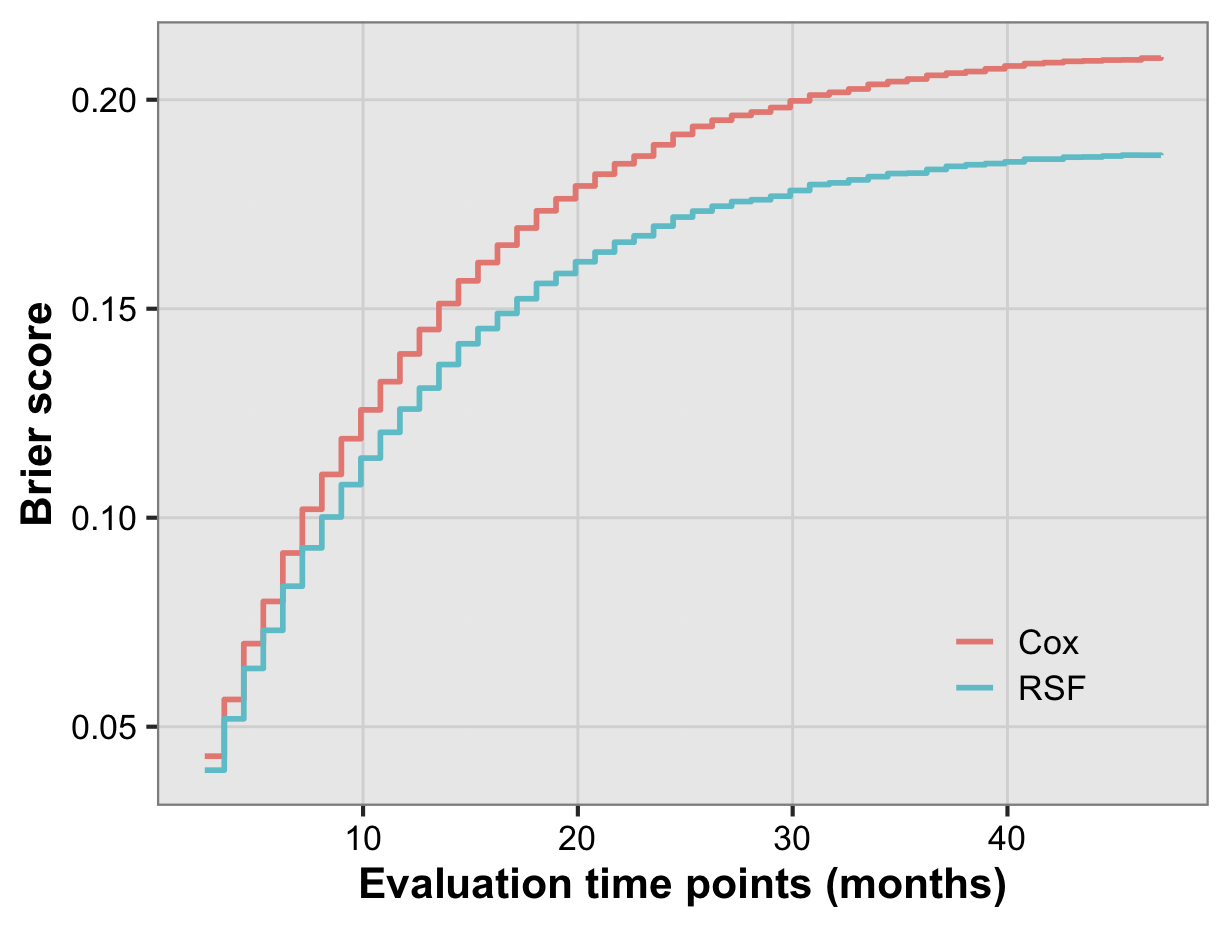
\includegraphics[width=0.8\linewidth]{figures/brierscore.png}
\caption{IPCW Brier score comparison between Cox and RSF models.}
\end{figure}

\begin{figure}[H]
\centering
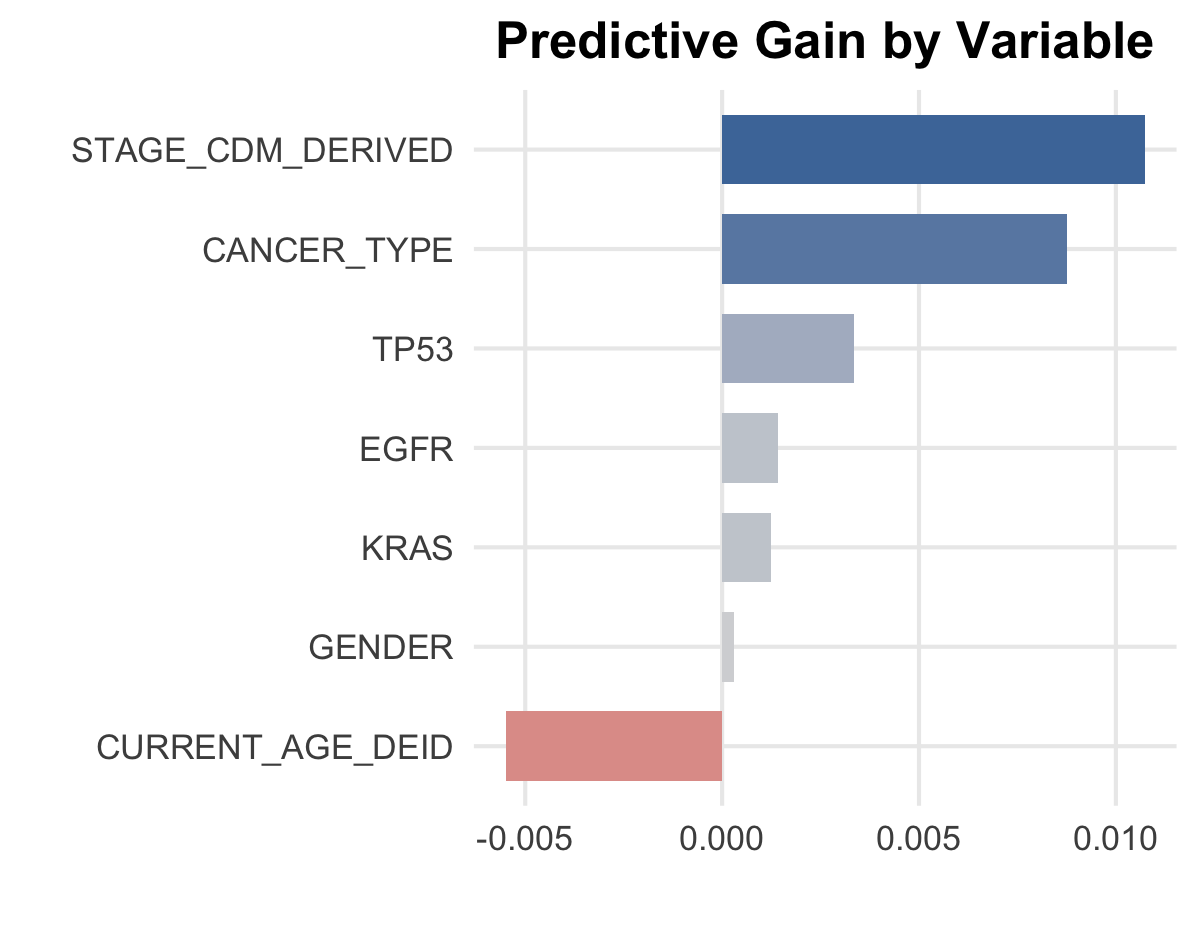
\includegraphics[width=0.8\linewidth]{figures/predictivegain.png}
\caption{Predictive gain of each variable based on integrated Brier score.}
\end{figure}

\begin{figure}[H]
\centering
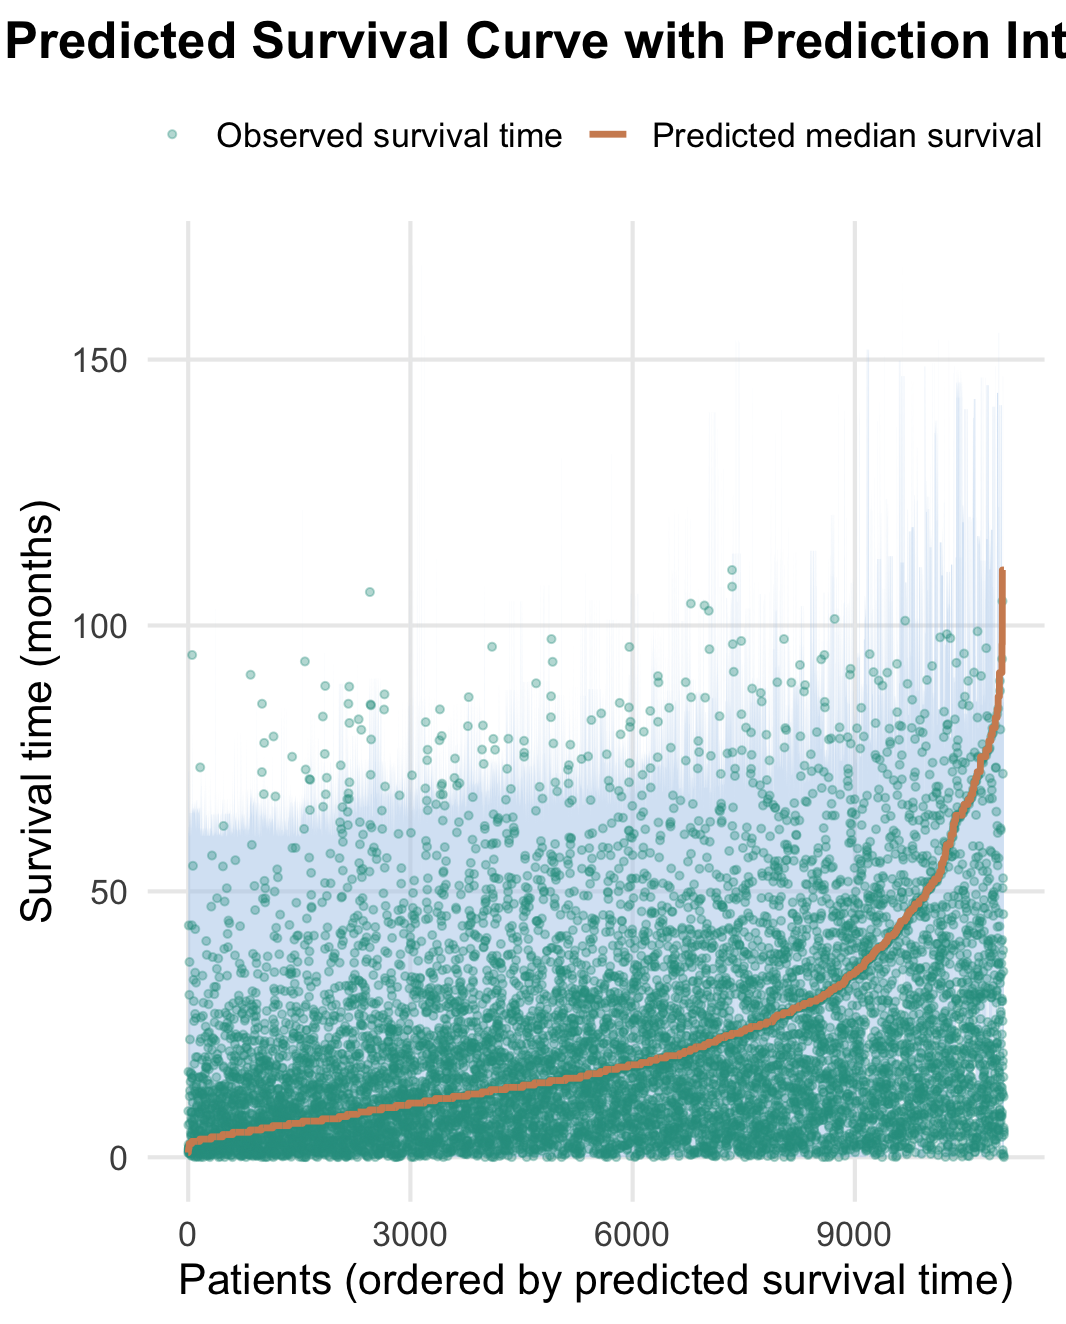
\includegraphics[width=0.85\linewidth]{figures/predictioninterval.png}
\caption{RSF predicted median survival time with prediction intervals.}
\end{figure}

\end{document}